\documentclass[10pt,twocolumn]{article}

\usepackage[letterpaper,top=.70in,bottom=.72in,left=.68in,right=.68in,columnsep=.26in,headheight=14pt]{geometry}
\usepackage{newpxtext,newpxmath}
\usepackage{microtype}
\usepackage{graphicx}
\usepackage{enumitem}
\usepackage{xcolor}
\usepackage{caption}
\usepackage{booktabs}
\usepackage{tabularx}
\usepackage[numbers,sort&compress]{natbib}
\usepackage{fancyhdr}
\usepackage{balance}
\usepackage{hyperref}

\definecolor{linkblue}{HTML}{244E6B}
\hypersetup{colorlinks=true,linkcolor=black,citecolor=black,urlcolor=linkblue,
  pdfauthor={Ashish Agrawal; Mukil Dharanidharan; Naman Upadhyay},
  pdftitle={Robust Defense Portfolios for Synthetic Hospital Ransomware Scenarios}}
\captionsetup{font=footnotesize,labelfont=bf,justification=raggedright,
  singlelinecheck=false,skip=4pt}
\setlength{\parindent}{1em}
\setlength{\parskip}{0pt}
\setlength{\emergencystretch}{2em}
\setlist{nosep,leftmargin=1.4em,topsep=2pt}
\setcounter{secnumdepth}{2}
\graphicspath{{../../results/figures/}}

\makeatletter
\renewcommand\section{\@startsection{section}{1}{0pt}{1.8ex plus .5ex}{.7ex}{\large\sffamily\bfseries}}
\renewcommand\subsection{\@startsection{subsection}{2}{0pt}{1.4ex plus .4ex}{.5ex}{\normalsize\sffamily\bfseries}}
\makeatother

\newcommand{\modelonly}{\textit{within the synthetic model}}
\newcommand{\codefield}[1]{\texttt{\detokenize{#1}}}

\pagestyle{fancy}
\fancyhf{}
\fancyhead[L]{\sffamily\scriptsize\MakeUppercase{Multi-objective hospital ransomware defense portfolios}}
\fancyhead[R]{\sffamily\scriptsize\thepage}
\renewcommand{\headrulewidth}{.35pt}
\renewcommand{\footrulewidth}{0pt}

\begin{document}

\twocolumn[
\begin{minipage}{\textwidth}
\small\sffamily\MakeUppercase{Paired multi-objective computational study}\hfill
Held-out confirmation; pre-predictive validation
\vspace{5pt}
\hrule
\vspace{12pt}
{\fontsize{20}{23}\selectfont\bfseries Robust Defense Portfolios for
Synthetic Hospital Ransomware Scenarios: A Paired Multi-objective Decision
Analysis with Held-out Confirmation\par}
\vspace{8pt}
{\normalsize Ashish Agrawal\textsuperscript{1} \quad
Mukil Dharanidharan\textsuperscript{1} \quad
Naman Upadhyay\textsuperscript{1}\par}
\vspace{2pt}
{\small\textsuperscript{1}Independent Student Researchers, Naperville, Illinois, USA\par}
\vspace{10pt}
\hrule
\vspace{8pt}
\small
\noindent\textbf{Abstract}\quad
Cyber-defense portfolios trade service continuity against implementation cost,
operational burden, and residual tail risk. Declaring one bundle ``best'' hides
those conflicts and can amplify Monte Carlo selection noise. We reformulated a
synthetic hospital ransomware model as a six-objective decision analysis. An
exact search enumerated 192 composable portfolios and collapsed configurations
that became behaviorally identical within each of three capacity profiles.
Every candidate in a profile replayed the same topology, entry point, patch
draws, and event-level random fields at five-minute resolution. The discovery
bank contained 12,960 executions (432 profile-candidates; 30 paired scenarios
each). Objectives were mean and worst-decile conditional mean weighted
service-hours lost, modeled sustained-outage probability, non-recovery by 72
hours, normalized implementation cost, and normalized operational burden.
Cost and burden were scenario points, not dollar or staffing estimates.

Discovery produced 55 point-estimate Pareto candidates. Before holdout
generation, we froze a finalist rule: at least 50\% bootstrap Pareto inclusion,
union all declared preference choices and benchmark strategies. This selected
57 profile-candidates, evaluated on 150 fresh paired scenarios each (8,550
executions). Forty-six of 52 discovery-frontier finalists remained
non-dominated: 22/28 in the resource-constrained profile and all 19/19 and 5/5
in the intermediate- and high-capacity profiles. No bundle minimized every
objective. Under declared budgets, preference-dependent choices differed by
profile; the strongest control stacks often exceeded the resource-constrained
and intermediate budgets. A public hospital-event dataset and CISA catalog
were retained as external construct checks, not used to fit control effects.
The framework supports auditable trade-off exploration \modelonly; it does not
estimate hospital risk or prove real-world control effectiveness.
\vspace{5pt}

\noindent\textbf{Keywords}\quad healthcare cybersecurity; ransomware;
multi-objective optimization; Pareto frontier; common random numbers; Monte
Carlo simulation; decision support; external validation
\vspace{12pt}
\end{minipage}
]

\section{Introduction}

Ransomware can interrupt care, displace demand to neighboring hospitals, and
extend recovery beyond restoration of a server. Among 374 publicly reported
attacks on U.S. healthcare delivery organizations from 2016 through 2021,
44.4\% mentioned care disruption and 41.7\% mentioned electronic-system
downtime \citep{neprash2022}. WannaCry was associated with lost appointments
and reduced activity at affected National Health Service trusts
\citep{ghafur2019}. A month-long U.S. attack was followed by increased demand,
longer waits, and stroke-care delays at neighboring emergency departments
\citep{dameff2023}; related work reported clinical changes at nearby,
unaffected hospitals \citep{pham2024,abouk2024}. These studies establish that
cyber incidents can become operational and regional events. They do not reveal
the counterfactual outcome of the same incident under a different defense
portfolio.

Simulation can replay a common latent incident, but a single-effectiveness
ranking creates another problem. Segmentation, patching, detection, isolation,
identity controls, and backup protection impose different costs and workflow
burdens. A portfolio that minimizes average disruption may be unattractive
under a small budget, have poor tail performance, or rely on aggressive
isolation. Multi-objective optimization addresses this by preserving
non-dominated alternatives instead of hiding preference choices inside one
score \citep{steuer1983,deb2002}. Cybersecurity investment research has also
treated defense selection as a constrained decision problem rather than a
one-dimensional ranking \citep{gordon2002,khouzani2019}.

Our previous analysis compared a flat reference with one layered portfolio.
It established an auditable paired workflow but also found that the estimated
effect changed with the simulation time step. The five-minute replication
preserved the direction, not the magnitude, and real data exposed missing
multi-hospital structure and an optimistic recovery pattern. Those findings
motivate a narrower and more defensible question:

\begin{quote}\itshape
Which defense portfolios remain Pareto-efficient across mean disruption, tail
disruption, modeled sustained outage, recovery, normalized cost, and normalized
operational burden when discovery choices are tested on fresh paired scenarios?
\end{quote}

We make three contributions. First, we correct the optimizer so every candidate
replays the same latent scenario bank. Second, we report a six-objective
frontier and explicit preference scenarios rather than a universal winner.
Third, we freeze finalist selection before a 150-scenario holdout. The study is
a computational decision analysis, not an empirical estimate of a hospital's
attack probability or control effectiveness.

\section{Methods}

\subsection{Synthetic model and control space}

The defensive Python model contains no malware, exploit code, scanning, or
connection to real infrastructure. A generated directed graph represents
permitted paths among workstations, electronic health record (EHR), laboratory,
pharmacy, imaging, medical-device, administrative, identity, backup, and
internet-facing/vendor functions. Nodes move among healthy, compromised,
detected, isolated, restoring, and restored states. Seven modeled services
depend on core and supporting nodes. Service availability is binary at each
step and therefore cannot represent degraded clinical operations.

The candidate vector contained six composable decisions: three segmentation
levels (flat, basic, least-privilege); zero to three patch-ladder upgrades;
faster detection; rapid same-step isolation; connected versus isolated backup;
and identity controls. Their Cartesian product generated 192 named portfolios.
Patch upgrades were capped at 90\%. Because different decisions can resolve to
the same effective settings when a profile already has a strong baseline, we
retained one representative for each resolved configuration. This yielded 192,
144, and 96 behaviorally distinct candidates in the resource-constrained,
intermediate-capacity, and high-capacity profiles, respectively.

The profile names are neutral scenario labels, not observed hospital classes.
They vary starting patch coverage, detection delay, isolation success, legacy
fraction, segmentation, backup connectivity, and a normalized budget. Their
budgets were 5, 10, and 15 points. The model ran for 864 five-minute steps (72
hours). Mechanistic rates were clock-time conversions of the frozen
five-minute replication protocol. They remain stress assumptions, not sector
estimates.

\subsection{Six decision objectives}

All objectives were minimized. We calculated them separately rather than
constructing one hidden utility function (Table~\ref{tab:objectives}).

\begin{table*}[t]
\centering
\caption{Decision objectives. Only simulated outcomes share units with the
model. Cost and burden are normalized scenario points.}
\label{tab:objectives}
\small
\begin{tabularx}{\textwidth}{@{}p{.22\textwidth}p{.29\textwidth}X@{}}
\toprule
Objective & Definition & Interpretation boundary \\
\midrule
Mean disruption & Mean weighted service-hours lost across seven binary modeled services & Expected within-model service unavailability; not patient harm \\
Tail disruption & Conditional mean loss among observations at or above the empirical 90th percentile (CVaR90) & Severity of the worst simulated decile \\
Sustained outage & Fraction of trials with more than two modeled hours of continuous unavailability in at least four clinical services & Model indicator; not an incident probability \\
Non-recovery & Fraction not technically recovered by the 72-hour horizon & Right-censored technical recovery, not return to normal operations \\
Implementation cost & Sum of declared control cost points & Relative scenario weight; not dollars or procurement evidence \\
Operational burden & Sum of declared workflow/implementation burden points & Scenario preference; not measured staff time \\
\bottomrule
\end{tabularx}
\end{table*}

We additionally retained defensive-isolation node-hours per node as a diagnostic
but did not add it as a seventh Pareto dimension. Cost weights were those
already declared in the repository. Burden weights were declared before this
analysis: basic and least-privilege segmentation 2 and 4 points; each patch
ladder step 3; faster detection 2; rapid isolation 3; protected backups 2; and
identity controls 3. Neither table is empirically calibrated. Every output
labels both as normalized points, and conclusions are restricted accordingly.

\subsection{Paired discovery design}

The earlier optimizer assigned a separate trial stream to each candidate,
allowing an easier random topology to influence the apparent winner. We
corrected the design. For every profile and replicate, all candidates reused
one flat base topology, nested patch draws, entry category and node, and
counter-style event-level random fields. Controls could delete or modify paths
but could not receive more favorable latent randomness. This is a common-random-
numbers design \citep{buffalo2026}.

Discovery used 30 paired scenarios for each of 432 profile-candidates: 12,960
executions. Entry categories cycled through workstation, internet-facing,
privileged-system, medical-device, and vendor-connection footholds. The exact
search evaluated every resolved candidate; it did not use a genetic or
surrogate optimizer. Point-estimate Pareto membership required that no other
candidate be no worse on all six objectives and strictly better on at least
one.

\subsection{Preference and benchmark rules}

The frontier is the primary result. To illustrate decisions, we declared four
weight sets: balanced; continuity-first; tail-risk-averse; and
resource-constrained. Within each profile's budget, objectives were min--max
normalized across feasible frontier points. We selected the minimum augmented
weighted Tchebycheff score: the worst weighted normalized shortfall plus 0.01
times the weighted sum. This form discourages weakly non-dominated compromises
and can represent discrete non-convex frontiers \citep{steuer1983}.

Four transparent comparators were retained: a zero-upgrade flat reference; the
prior layered heuristic (basic segmentation, faster detection and rapid
isolation, isolated backup); the maximum-control stack; and the candidate with
the largest mean service-hours preserved per cost point within the profile
budget. ``Heuristic'' denotes a reproducible rule, not expert endorsement.

\subsection{Bootstrap stability and frozen holdout}

Discovery-frontier stability used 500 paired scenario bootstraps. Each
resample drew whole scenario identifiers with replacement and carried every
candidate response for that scenario, preserving cross-portfolio correlation.
All six objectives and the frontier were recomputed. Before generating holdout
data, we wrote a protocol containing the exact rule, identities, seed, and
sample size. A finalist entered if its bootstrap Pareto-inclusion probability
was at least 0.50, or if it was selected by any declared preference or benchmark
rule. The union contained 57 profile-candidates: 29 resource-constrained, 21
intermediate-capacity, and 7 high-capacity.

Each finalist then ran on 150 fresh paired scenarios with a new master seed,
producing 8,550 holdout executions. The holdout frontier used the same
definitions, with 1,000 paired bootstraps. No candidate was added or removed
after holdout outcomes were observed.

\subsection{Observed-data bridge}

Observed records were kept outside the optimizer. The public THREAT replication
deposit \citep{neprashdata2025} was normalized from its displayed public
preview, deduplicated by Medicare identifier, THREAT identifier, and attack
date, and yielded 149 attacked hospital-event records across 74 events from
2016 through 2021. Emergency-diversion and cancellation/delay flags occurred in
46/149 (30.9\%) and 73/149 (49.0\%) records; 19/74 events involved multiple
hospitals. The associated claims study estimated a 17--24\% decline in hospital
volume in the first attack week with recovery over roughly three weeks
\citep{neprash2026}.

We also froze CISA's Known Exploited Vulnerabilities catalog at version
2026.09.01 \citep{cisakev2026}. It contained 1,687 records, including 352 tagged
for known ransomware use. These sources support event timing, breadth,
operational relevance, and vulnerability provenance. They do not identify
per-edge spread, control effects, hospital exposure, procurement cost, or
workflow burden. We therefore used them as construct and structural checks,
not as calibration targets or optimization objectives.

\subsection{Reproducibility and verification}

Raw discovery and holdout trials, objective summaries, frontier membership,
preference choices, bootstrap inclusion frequencies, protocol manifests,
configuration, burden weights, source snapshots, and plotting scripts are
versioned. Seventy automated tests cover transitions, pairing, budgets,
derived metrics, observed-data processing, Pareto dominance, CVaR, burden
calculation, finalist union, and holdout pairing. The reporting follows the
transparency intent of the STRESS simulation guidelines \citep{monks2019}.

\section{Results}

\subsection{Discovery and held-out frontiers}

Discovery identified 55 point-estimate Pareto candidates: 31, 19, and 5 in the
resource-constrained, intermediate-capacity, and high-capacity profiles. After
the frozen finalist rule and fresh evaluation, the holdout contained 49
non-dominated candidates: 22 of 29 tested resource-constrained candidates, 20
of 21 intermediate candidates, and all 7 high-capacity candidates. Bootstrap
Pareto inclusion was at least 0.80 for 21, 16, and 7 candidates, respectively.
The large frontier is not evidence that all portfolios are equally useful. It
shows that six objectives create genuine and sometimes small trade-offs.

Among 52 tested candidates that had been on the discovery point frontier, 46
remained on the holdout frontier (Figure~\ref{fig:survival}). Survival was
22/28 (78.6\%) in the resource-constrained profile and 19/19 and 5/5 in the
intermediate- and high-capacity profiles. The six dropped candidates are
treated as discovery artifacts, not hidden.

\begin{figure}[t]
\centering
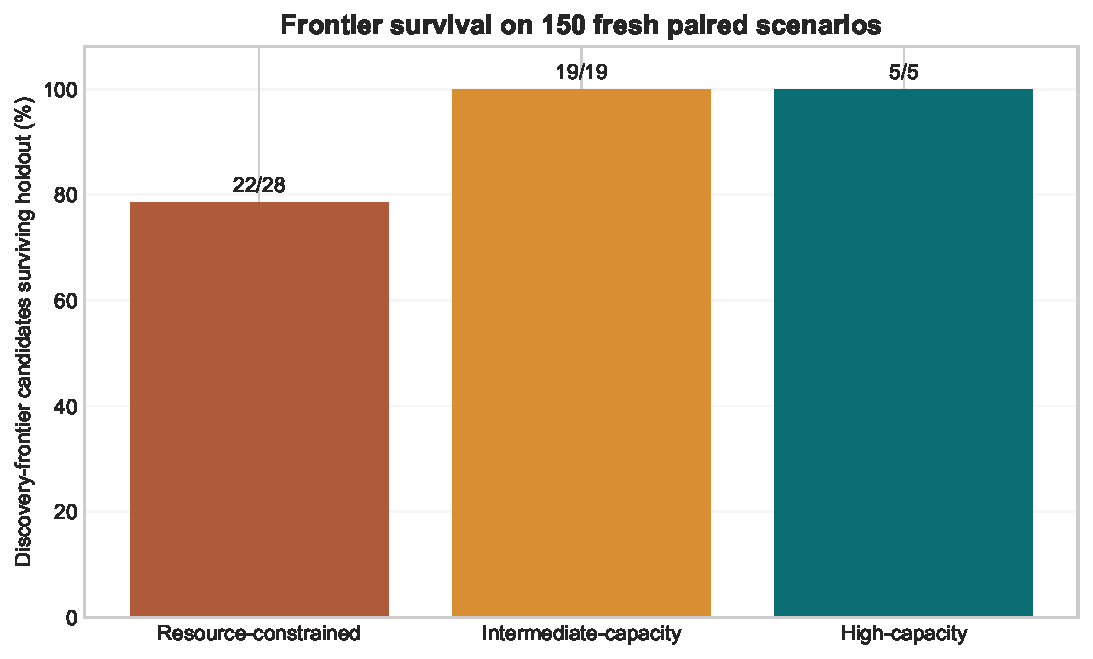
\includegraphics[width=\columnwidth]{multiobjective_discovery_holdout_survival.pdf}
\caption{Discovery-frontier survival on 150 fresh paired scenarios per
finalist. Numerators are candidates that remained non-dominated; denominators
are discovery-frontier candidates admitted to holdout.}
\label{fig:survival}
\end{figure}

\subsection{Trade-offs and budget constraints}

No candidate minimized all six objectives. Figure~\ref{fig:frontier} projects
the held-out frontier onto normalized cost and mean disruption; color shows the
modeled sustained-outage probability and point size shows bootstrap stability.
In the resource-constrained profile, the declared five-point budget intersects
the frontier while mean loss and sustained-outage probability remain high.
Large modeled improvements require portfolios outside that budget. The
intermediate profile shows a steep improvement between 5 and 10 points and
further reductions beyond budget. In the high-capacity profile, much of the
modeled performance gain occurs by three to six points and additional controls
offer smaller changes.

\begin{figure*}[t]
\centering
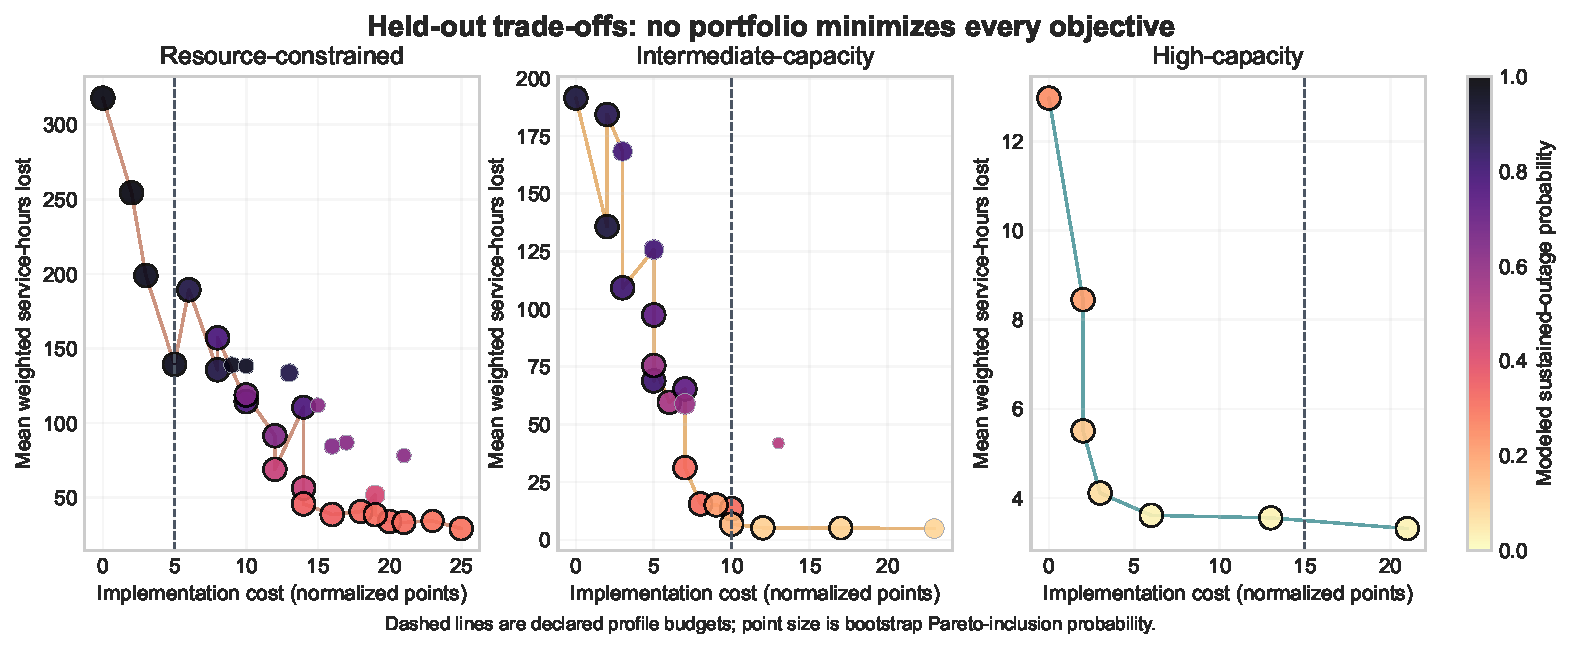
\includegraphics[width=\textwidth]{multiobjective_holdout_frontier.pdf}
\caption{Held-out profile-specific trade-offs. Lines connect non-dominated
points in the cost--mean-loss projection, not a one-dimensional ranking.
Dashed lines are declared profile budgets. Costs are normalized points, not
dollars.}
\label{fig:frontier}
\end{figure*}

The declared preference rules selected different portfolios (Table
\ref{tab:preferences}). Under the resource-constrained five-point budget, the
continuity and tail-risk rules selected faster detection plus isolated backup;
mean loss was 139.3 weighted service-hours, but sustained-outage probability
remained 95.3\%. The resource-focused rule selected isolated backup alone and
accepted higher mean loss (254.4 hours). Under the intermediate ten-point
budget, the tail-risk rule selected least-privilege segmentation, one patch
upgrade, and faster detection; mean loss was 6.8 hours, CVaR90 was 34.4, and
sustained-outage probability was 15.3\%. Under the high-capacity budget, the
continuity rule selected basic segmentation plus faster detection; mean loss
was 3.6 hours and sustained-outage probability was 2.7\%. These are conditional
model outputs, not expected hospital outcomes.

\begin{table*}[t]
\centering
\caption{Selected held-out preference examples. Portfolio labels are expanded
for readability; all choices satisfy the declared profile budget.}
\label{tab:preferences}
\small
\begin{tabularx}{\textwidth}{@{}p{.16\textwidth}p{.15\textwidth}Xrrrr@{}}
\toprule
Profile & Preference & Selected controls & Cost & Mean loss & CVaR90 & Outage \\
\midrule
Resource-constrained & Continuity / tail & Faster detection; isolated backup & 5 & 139.3 & 218.3 & 95.3\% \\
Resource-constrained & Resource-focused & Isolated backup & 2 & 254.4 & 330.9 & 97.3\% \\
Intermediate & Balanced & Basic segmentation; faster detection & 6 & 59.6 & 171.5 & 54.7\% \\
Intermediate & Continuity & Least privilege; faster detection & 8 & 15.5 & 79.1 & 31.3\% \\
Intermediate & Tail-risk & Least privilege; one patch step; faster detection & 10 & 6.8 & 34.4 & 15.3\% \\
High-capacity & Continuity / tail & Basic segmentation; faster detection & 6 & 3.6 & 17.5 & 2.7\% \\
\bottomrule
\end{tabularx}
\end{table*}

\subsection{Benchmark strategies}

The maximum-control stack had the lowest mean benchmark loss in each profile,
but it cost 25, 23, and 21 points and exceeded every declared budget. The
layered heuristic cost 13 points; it was affordable only in the
high-capacity profile. Relative to the flat reference, the layered heuristic
reduced held-out mean loss from 317.9 to 133.6 hours in the
resource-constrained profile, 191.5 to 41.9 in the intermediate profile, and
13.0 to 3.6 in the high-capacity profile (Figure~\ref{fig:benchmarks}). Its
worst-decile conditional means remained 208.9, 141.7, and 17.5 hours. The
result is therefore not ``the layered portfolio wins''; it is that performance,
tail risk, and feasibility move differently across profiles.

\begin{figure*}[t]
\centering
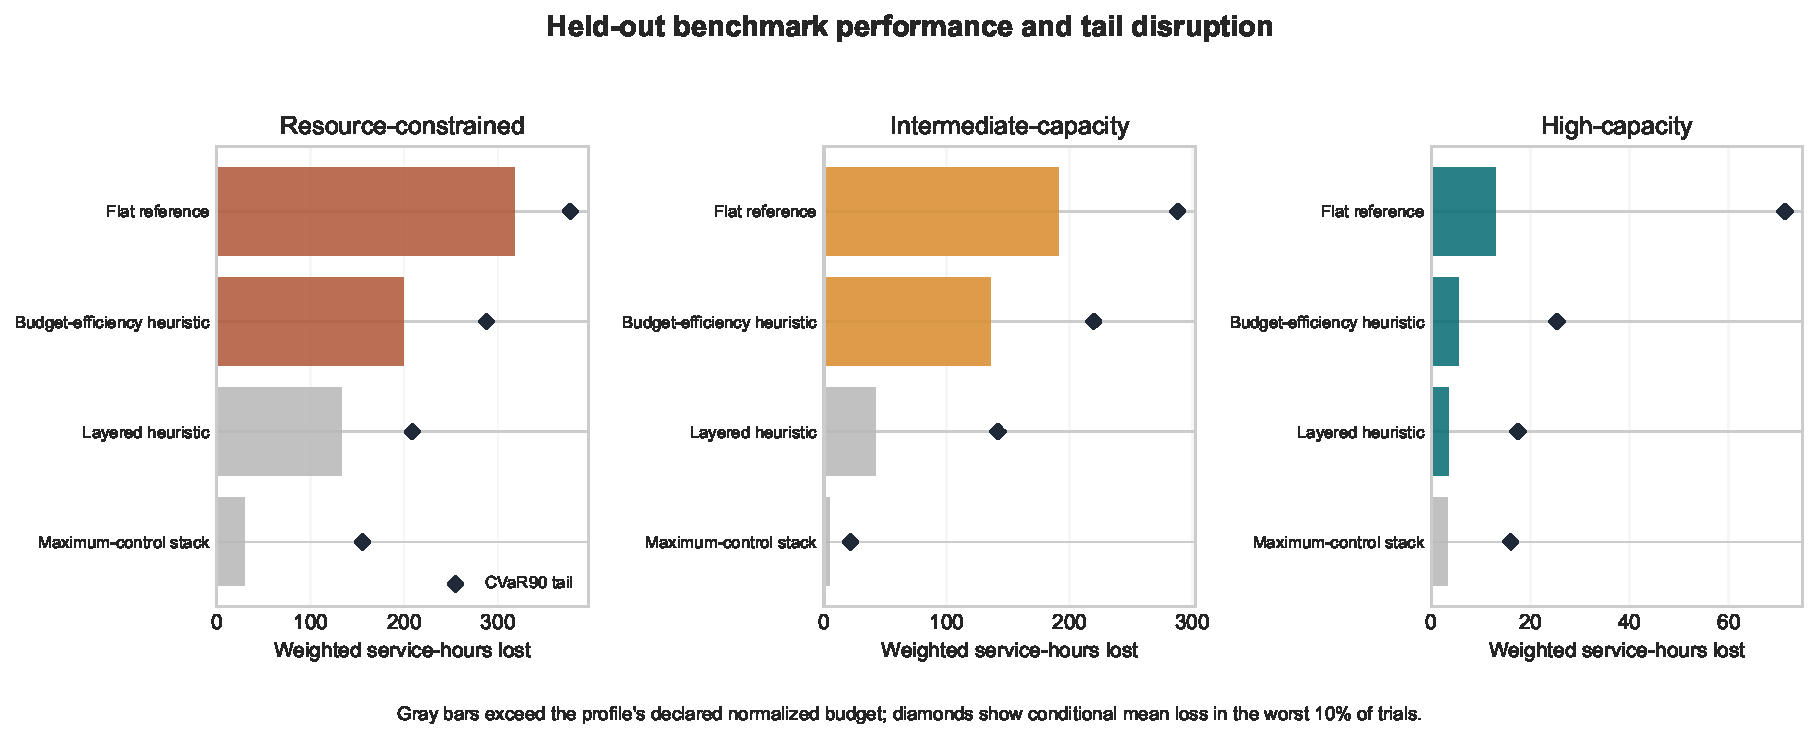
\includegraphics[width=\textwidth]{multiobjective_holdout_benchmarks.pdf}
\caption{Held-out benchmark strategies. Bars show mean weighted service-hours
lost; diamonds show CVaR90. Gray strategies exceed the profile budget. The
maximum-control stack is an unconstrained comparator, not a recommendation.}
\label{fig:benchmarks}
\end{figure*}

\subsection{What the observed data did and did not validate}

The observed sources did not validate a portfolio ranking. They instead
defined failure boundaries. The simulator has one facility per run, whereas
25.7\% of THREAT events involved multiple Medicare hospitals. Its binary
service-hours cannot be converted into diversion or canceled care. Technical
reference recovery occurs much earlier than the roughly three-week
hospital-volume pattern. CISA provides real exploited-vulnerability identities
but not a hospital attack probability or patch-effect estimate. Consequently,
none of the six objectives is an empirically calibrated hospital outcome, cost,
or burden measure. The study remains pre-predictive validation.

\section{Discussion}

\subsection{Principal finding}

The central result is methodological: after pairing candidates, separating six
objectives, and using fresh holdout scenarios, there is no universal portfolio
winner. The apparently simple question ``which bundle is best?'' requires a
budget and preferences over average disruption, tail disruption, sustained
outage, recovery, cost, and burden. A single score can still be useful, but its
weights are a decision input, not a scientific finding.

The holdout also changes how uncertainty is communicated. Forty-six of 52
discovery-frontier candidates survived, but six resource-constrained candidates
did not. Bootstrap inclusion probabilities further distinguish persistent
trade-offs from fragile point estimates. This is more informative than naming
the minimum sample mean, whose old reselection rate ranged from 1.4\% to 100\%
across profile-budget cells.

\subsection{Interpretation by capacity profile}

The resource-constrained scenario presents the hardest decision. Its five-point
budget cannot buy the modeled combinations that substantially reduce sustained
outage. The honest conclusion is not that isolated backup plus faster detection
is sufficient; it is the least-bad continuity compromise among the modeled
feasible options under one declared preference. The intermediate scenario
shows a consequential choice between cheaper detection-oriented bundles and a
ten-point least-privilege/patch/detection bundle. The high-capacity scenario
exhibits diminishing modeled gains: a smaller bundle performs near the
maximum-control stack on mean loss, while preserving cost and burden.

These patterns are useful for tabletop exploration: they reveal where a
decision hinges on budget or preference. They cannot determine how a hospital
should spend money because normalized costs omit procurement, integration,
training, maintenance, alert workload, and constraints unique to clinical
technology.

\subsection{Strengths and limitations}

Strengths include exact enumeration, behavior-based deduplication, common
random numbers, a frozen five-minute protocol, six separately reported
objectives, declared weights, discovery/holdout separation, paired bootstrap
stability, raw-data retention, and an observational bridge that is allowed to
contradict the model. The pipeline does not use observed outcomes to tune an
answer.

The main limitation is external validity. Topology, transition hazards,
service dependencies, control effects, cost, and burden are not jointly
observed in real hospitals. A binary service threshold omits degraded work,
patient flow, manual workarounds, staffing, and regional spillover. Technical
recovery is not operational recovery. The six-dimensional frontier can also be
large because dominance becomes less common as objectives are added; bootstrap
stability mitigates but does not eliminate this many-objective effect. The
150-scenario holdout estimates within-model behavior, not real effectiveness.

The THREAT CSV is normalized from a public preview because original-file
download requires ICPSR sign-in. The original file and codebook should replace
it before submission, with reconciliation recorded. Zero operational flags may
mean ``not reported.'' The CISA catalog is curated and its ransomware-tagged
share is not a base rate. Normalized cost and burden weights require independent
sensitivity analysis and domain review before decision use.

\subsection{Next validation step}

The next study should not add simulations first. It should obtain domain and
empirical inputs: structured review by hospital IT/security and clinical-
operations staff; defensible control-cost and workload ranges; and longitudinal
incident or exercise data containing service state and recovery over time. A
future protocol should calibrate on one time period or site set, lock the model,
and evaluate prediction on held-out incidents. Multi-hospital structure and
continuous-time dynamics should be added before claiming regional or exact
clock-time performance.

\section{Conclusion}

We transformed a one-comparison simulation into a paired, six-objective
portfolio decision analysis with a frozen holdout. Across 21,510 new
executions, many defense portfolios remained non-dominated and no bundle
minimized every objective. Stronger stacks often reduced modeled disruption
but exceeded declared budgets; feasible preference choices differed sharply by
capacity profile. Forty-six of 52 discovery-frontier finalists remained
non-dominated on fresh scenarios, while six resource-constrained candidates
dropped out.

The defensible contribution is not a defense portfolio that ``beats
everything.'' It is a reproducible method for exposing trade-offs, selection
instability, budget infeasibility, and model failure boundaries. The outputs
can support research and tabletop discussion \modelonly. They should not be
used as hospital risk estimates, procurement recommendations, or evidence that
a deployed control will achieve the reported hours or probabilities.

\section*{Research integrity and declarations}

\textbf{Ethics.} The study used synthetic networks, simulated trajectories,
public organization-level hospital-event records, a public vulnerability
catalog, and published aggregate findings. It involved no participants,
patient-level records, private organizational data, malware, or intervention.
External interviews have not been conducted. Consent, privacy, and
institutional requirements must be reviewed before future human-participant or
organizational data collection.

\textbf{Data and code.} Code, configuration, raw simulation outputs, public
observed-data snapshots, processed tables, figures, tests, and manifests are at
\url{https://github.com/Dodgeboi/NazeResearchNSRI}. A submitted version should
cite a fixed release or archived commit.

\textbf{Artificial-intelligence use.} Claude, ChatGPT, and Codex were used for
coding assistance, debugging ideas, literature-search terms, analysis checks,
organization, and editing suggestions. Their responses were not treated as
evidence. Numerical claims were checked against committed data and code, and
literature claims against cited sources. The authors remain responsible for
the analysis and wording.

\textbf{Author contributions.} Ashish Agrawal, Mukil Dharanidharan, and Naman
Upadhyay developed the project and reviewed the manuscript. Detailed CRediT
roles should be agreed before formal submission.

\textbf{Funding.} The authors report no specific funding for this work.

\textbf{Conflicts of interest.} The authors report no known competing
interests. All authors should reconfirm this statement before submission.

\bibliographystyle{unsrtnat}
\renewcommand{\bibfont}{\footnotesize}
\setlength{\bibsep}{0.5pt}
\bibliography{references}

\end{document}
